\documentclass[conference]{IEEEtran}
\usepackage[T1]{fontenc}
\usepackage{booktabs,amsmath,url,balance,graphicx}
\usepackage{pgfplots,tikz}
\pgfplotsset{compat=1.18}
\title{Processing Controls and Calibration for Watermarks and AI Image Detection}
\author{\IEEEauthorblockN{Anonymous Authors}}
\begin{document}\maketitle
\begin{abstract}
On a prospectively locked caption-paired test with shared final encoding,
frozen ResNet and CLIP probes achieve AUCs of 0.729 and
0.820, substantially below their collection-based results.
A same-source, equal-size factorial separately estimates transformation-matching
gains of 0.0056 and 0.0050.
Equal-slot controls show that training-row count alone does not explain
the larger augmentation gains. We evaluate passive origin detection and
expected-payload scores under shared edits, using an agreement gate that
returns the probe score when recovery is weak. Independent fusion fitting
and calibration quantify the cost of controlling false alarms. Conservative
source-level cuts reduce recall and require exchangeable sources within the
stated processing family. Classical and learned marks share information bits,
matched embedding distortion, and common nominal false-match targets.
The contribution is a reproducible set of controls for processing, content,
fusion, and calibration. The results support conditional fusion benefits
and demonstrate limits to cross-pipeline detection and watermark recovery
within the tested models and collections.
\end{abstract}
\begin{IEEEkeywords}
AI image detection, digital watermarking, image forensics, calibration
\end{IEEEkeywords}

\section{Introduction}
An origin detector estimates resemblance to a synthetic training class;
a watermark detector checks an expected embedded payload. Compression,
cropping, and resampling affect both. Prior work studies shared degradations
and cross-generator transfer \cite{univfd,genimage}; reconstruction and
adaptive attacks can remove watermark evidence \cite{zhao,unmarker}.
We ask which benefits survive controls for training information, source
content, and decision calibration (Fig.~\ref{fig:pipeline}). Contributions are:
\begin{itemize}
\item A same-source factorial test isolating a modest transformation-matching
interaction from augmentation-set main effects across repeated splits.
\item Agreement-gated fusion with marked/unmarked controls, and independently
calibrated image- and source-level operating points.
\item A locked caption-paired evaluation with shared encoding and a watermark
comparison with common information bits, distortion, and false-match targets.
\end{itemize}

\section{Related Work}
Frozen-CLIP transfer \cite{univfd}, GenImage's degradation tests
\cite{genimage}, CNNDetection's augmentation \cite{cnndetect}, DIRE's
reconstruction error \cite{dire}, and CIFAKE \cite{cifake} inform passive
detection. Generative reconstruction \cite{zhao}, UnMarker \cite{unmarker},
latent diffusion \cite{ldm}, and SDEdit \cite{sdedit} inform removal.
TrustMark is a learned post hoc mark \cite{trustmark}; Stable Signature
modifies the decoder \cite{signature}, and Tree-Rings modifies generation
noise \cite{treering}. DWT/DCT are established components \cite{alhaj}.
AdvMark optimizes embedding for detectability \cite{advmark}.
NIST distinguishes provenance from authenticity
\cite{nist}.

\section{Data and Experimental Design}
We use \emph{Experiment 1: core}, \emph{Experiment 2: encoding and fresh
sample}, and \emph{Experiment 3: learned mark}.
\begin{figure*}[t]
\centering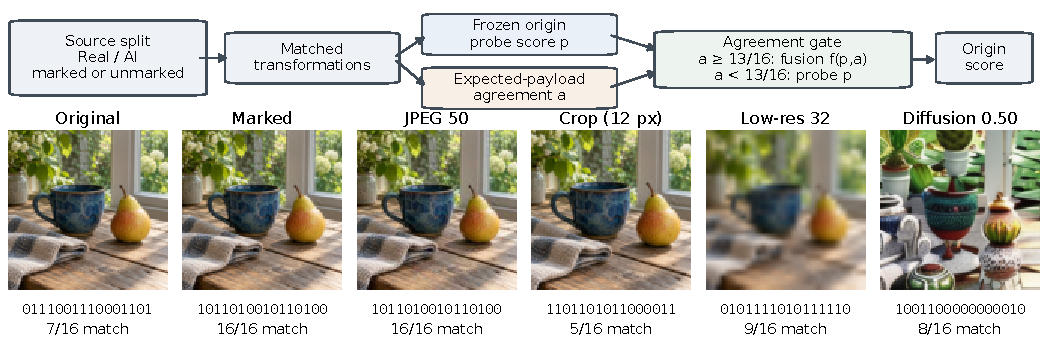
\includegraphics[width=\textwidth]{assets/pipeline_examples.pdf}
\caption{Pipeline and a project-generated illustration processed by the
actual classical watermark and attacks. Recovered bits and agreement with
\texttt{1011010010110100} appear below each image. The illustration is excluded
from every benchmark; diffusion uses strength 0.50.}
\label{fig:pipeline}\end{figure*}

\subsection{Collections and source splits}
The original selection contains 2,000 COCO photographs \cite{coco},
2,000 DiffusionDB images \cite{diffusiondb}, 1,000 DALL$\cdot$E~3-labeled
images \cite{dalle}, and 1,000 Midjourney-labeled images \cite{midjourney}.
Release-prefix selection replaces short sides below 256. Synthetic exports
receive JPEG95; COCO retains its encoding. Area-resized $256\times256$
pixels are staged as PNG. Experiment~2 applies common final JPEG encoding.

The original stratified split uses 0.70/0.15/0.15 for seen collections;
Midjourney is test-only. An audit/refit retains one representative from
native/standardized exact-pixel or $8\times8$ average-hash components
(Hamming distance $\le2$), preferring train, validation, then test.
It excludes 177 sources and retains 5,823 (Table~\ref{tab:sources}).
\begin{table}[t]
\caption{Original retained sources. SD: DiffusionDB. Repeated splits additionally
use 1,000 screened Open Images photographs.}
\label{tab:sources}\centering\small
\begin{tabular}{lrrrr}\toprule
Split & COCO & SD & DALL$\cdot$E 3 & Midjourney\\\midrule
Train & 1345 & 1370 & 700 & 0\\
Validation & 291 & 292 & 145 & 0\\
Test & 284 & 300 & 134 & 962\\
\bottomrule\end{tabular}\end{table}

Clean/edited/opposite-payload real rows are R-C/R-T/R-S; unmarked/marked/
edited-marked AI rows are S-U/S-W/S-A. Derivatives inherit source splits;
processing and seeded noise match across origins. Original tests have
sixteen copies per source. Adding fourteen unmarked AI edits gives
46,424 copies with original heads fixed. Adding Open Images
\cite{openimages}, seeds 20260920--20260924 each have
4,102/878/1,843 training/validation/test sources; every test has 49,158
copies, thirty/sixteen per AI/real source. Supervised fitting uses thirteen
conditions; three weak settings are withheld from fitting. Midjourney never
enters fitting.

\subsection{Training and calibration controls}
Equal-size controls replace each real source's eleven R-T slots with its
clean feature or six JPEG70/five JPEG50 features: 53,326 rows per arm,
identical sources, labels, class weights, and optimization.
The unmarked factorial instead crosses real/AI edit sets
$A=\{\mathrm{JPEG70},\mathrm{blur3}\}$ and
$B=\{\mathrm{noise6},\mathrm{resize0.8}\}$. Each source supplies clean plus
two augmented rows. Available caches restrict synthetic fitting to 1,834
non-Midjourney sources; all 1,843 test sources remain. Each arm has identical
within-split sources/rows and is tested on clean plus all four edits
(9,215 copies). The planned contrast is
\begin{equation}\Delta_{\rm match}=\tfrac12(AUC_{AA}+AUC_{BB}-AUC_{AB}-AUC_{BA}).\end{equation}

For each split, unchanged full probes use 439 validation sources for new
fusion fitting and 439 disjoint sources for calibration, including 144 COCO
and 75 Open Images photographs. Additional seed-20260920 heads exclude SD
and Midjourney from every supervised fitting stage; their synthetic training
class contains DALL$\cdot$E~3 only.

\subsection{Experiments 2 and 3}
Experiment~2 uses 300 approximately CLIP-paired real/AI pairs (600 sources),
a frozen 192-source sample, and a locked 400-source replication (80 per
collection). Its identity/JPEG50/crop/low-res32 marked/unmarked AI and shared
JPEG95 yield 2,560 copies. New calibration reanalysis is a follow-up.
UniversalFakeDetect uses its released head and official native-image
224-pixel center crop.

The new content control fixes 200 unused COCO photograph/caption pairs.
Photographs exclude prior public IDs and exact/hash overlaps before generation.
One image per caption uses Realistic Vision V5.1 with official
LCM-LoRA \cite{lcm}, eight steps, guidance one, $512\times512$, fixed
ID-derived seeds, and no candidate resampling. Both origins receive area
resize to $256\times256$/JPEG95, followed by identity, JPEG50, or low-res32 (1,200 unmarked
copies). Head/threshold/asset locks precede generation and one inference pass.

Experiment~3 retains 204 AI sources, 68 per generator, and three balanced
payloads. The fair comparison adds 400 calibration and 400 test photographs,
200 COCO/200 Open Images each, screened for overlap across arms.
Both marks encode sixteen information bits under identity/JPEG50/crop/low-res32.
Whole-residual scaling and identically seeded stochastic pixel rounding
match PSNR to $40\pm0.1$\,dB before decoding; this is a modified embedding
configuration for both methods. Official TrustMark 0.9.2 Q uses BCH5,
sixteen data bits plus 45 zeros. Sources are reused diagnostic items.

\section{Methods}
\subsection{Watermark and transformations}
The classical mark applies Haar luminance decomposition and DCT to
$8\times8$ LL tiles. Coefficients $(3,2)$ and $(2,3)$ have difference
$12(2b-1)$ for repeated payload bit $b$; median differences decode bits.
Agreement $a$ compares with \texttt{1011010010110100}; original embedding
PSNR averages 40.1\,dB on 3903 AI sources.
Seen edits are JPEG70/50, blur kernels 3/5, noise $\sigma=6$, resize to 80\%,
crop twelve pixels per side, saturation$\times1.08$/value$\times0.95$,
nonlocal means ($h=h_{color}=5$, windows 7/21), centered radius-16 Telea
inpainting (radius 3), and a $64\times64$ round trip.
Withheld edits are low-res32 (a $32\times32$ round trip), a seven-pixel circular shift plus JPEG19 and
noise $\sigma=16$, and an LL-tile spectral wipe ($2\le i+j\le5$).
Area downsampling and linear restoration are fixed. The grid shift is not
diffusion regeneration.

\subsection{Probes, fusion, and calibration}
Frozen ImageNet ResNet-18 \cite{resnet} and OpenAI CLIP ViT-B/32
\cite{clip} provide 512-dimensional features. ResNet uses ImageNet-normalized
224-pixel inputs; CLIP uses official preprocessing and OpenCLIP GELU.
Balanced L2 logistic probes use $C=1$, LBFGS and 3,000 maximum iterations;
all new fits converge.
For probe probability $p$ and classical payload agreement $a$, independently fitted
fusion and the gate are
\begin{equation}
f=\sigma(\beta_0+\beta_p p+\beta_a a),\qquad
g=\begin{cases}f,&a\ge13/16,\\p,&a<13/16.\end{cases}
\end{equation}
The agreement cut was selected on original validation and retained throughout.
Original fits
reuse validation for fusion and threshold selection; new fits/calibration
use disjoint source halves. Test ROC ranks logits. TPR$_5$ denotes a
test-ROC diagnostic, not a deployed threshold.

Image calibration chooses the lowest real-copy threshold with FPR$\le0.05$
and accepts scores$\ge$threshold with whole ties. Source calibration ranks each
photograph's maximum over the fixed processing family. In each collection,
$k=\lceil(n+1)(1-0.05)\rceil$ selects the $k$th ascending maximum among $n$
sources; acceptance requires strict exceedance. The global cut is the larger
COCO/Open Images cut. Thirteen-/sixteen-condition cuts precede testing.
This split-conformal adaptation \cite{conformal} is marginal under
collection/family exchangeability; realized-split or unseen-shift guarantees
do not follow.

Watermark scores average signed expected-bit margins: classical median
differences/12 or TrustMark's first sixteen raw pre-ECC logits. Default and
maximum-over-three cuts target nominal 5\% using calibration photographs
only. These margins are not official message probabilities;
exact-message/ECC and $\ge13/16$ recovery are secondary.

\subsection{Statistical reporting}
Source bootstraps retain derivatives and shared comparison draws. Overlapping
splits make mean$\pm$SD a sensitivity measure. Factorial/calibration/caption-pair
analyses use 2,000/1,000/2,000 draws; watermark draws preserve collection
strata. Within-collection binomial bounds assume independent common-risk
sources and supplement zero events, whose ordinary bootstrap is degenerate.
Test thresholds remain fixed.

\section{Results}
\subsection{Transformation matching}
Equal-size full-minus-clean-repeat AUC is 0.0467 [0.0435,0.0501] for
ResNet and 0.0147 [0.0133,0.0163] for CLIP; full-minus-JPEG-only gain is
0.0303/0.0122. The factorial isolates a smaller matching interaction
(Table~\ref{tab:factorial}): 0.0056 [0.0050, 0.0062] and
0.0050 [0.0044, 0.0056]. Fixed-validation TPR interactions are
0.0182/0.0238, while FPR-interaction intervals cross zero.
\begin{table}[t]
\caption{Unmarked same-source factorial, mean$\pm$SD across five splits.
Rows match sources, slots, weights and optimization within each split.}
\label{tab:factorial}\centering\footnotesize
\begin{tabular}{lcc}\toprule
Real/AI edit set & ResNet AUC & CLIP AUC\\\midrule
A/A & $0.926\pm0.002$ & $0.991\pm0.001$\\
A/B & $0.921\pm0.003$ & $0.987\pm0.002$\\
B/A & $0.922\pm0.003$ & $0.987\pm0.001$\\
B/B & $0.927\pm0.002$ & $0.992\pm0.001$\\
\bottomrule\end{tabular}\end{table}

\subsection{Fusion and reduced payload recovery}
With original heads fixed, adding unmarked AI edits gives ResNet
probe/fusion/gate AUC 0.942/0.939/0.954 and CLIP 0.994/0.988/0.994.
Marked-minus-unmarked ResNet probability change is 0.0022 [0.0008,0.0036];
fixed-threshold TPR change has interval [-0.0017,0.0032].
Original payload acceptance is 1.000 on clean marked AI,
0.710 on edited marked AI, and 0.0075 on real copies.
In Table~\ref{tab:attacks}, crop agreement averages 0.488/0.515
for AI/real, with expected-payload AUC 0.437 [0.401,0.473]; chance-like means
need not imply identical distributions. Across the four weak settings, ResNet
probe/fusion/gate AUC is 0.922/0.882/0.923;
CLIP is 0.988/0.957/0.988.
\begin{table}[t]
\caption{Original matched conditions. Bits: marked-AI agreement; active:
payload AUC; P/F/G: ResNet probe/fusion/gate AUC. Identity compares
S-W/R-C; edits compare S-A/R-T. Bold: weak recovery. Star: withheld fitting.}
\label{tab:attacks}\centering\footnotesize\setlength{\tabcolsep}{3pt}
\begin{tabular}{lrrrrr}\toprule
Transformation & Bits & Active & P & F & G\\\midrule
Identity & 1.000 & 1.000 & 0.952 & 0.993 & 0.981\\
JPEG 70 & 0.999 & 1.000 & 0.946 & 0.994 & 0.977\\
JPEG 50 & 0.985 & 0.997 & 0.947 & 0.992 & 0.970\\
Blur, kernel 3 & 0.995 & 1.000 & 0.954 & 0.995 & 0.980\\
Blur, kernel 5 & 0.985 & 0.999 & 0.953 & 0.994 & 0.979\\
Noise, $\sigma=6$ & 0.999 & 1.000 & 0.954 & 0.995 & 0.987\\
Resize, 80\% & 0.995 & 1.000 & 0.954 & 0.995 & 0.981\\
\textbf{Crop, 12 px/side} & \textbf{0.488} & \textbf{0.437} & \textbf{0.957} & \textbf{0.909} & \textbf{0.957}\\
Color & 0.999 & 1.000 & 0.953 & 0.994 & 0.980\\
Denoise & 0.963 & 0.993 & 0.936 & 0.986 & 0.964\\
Inpaint & 1.000 & 1.000 & 0.950 & 0.992 & 0.982\\
Low-res 64 & 0.949 & 0.997 & 0.941 & 0.993 & 0.974\\
\textbf{Low-res 32$^\star$} & \textbf{0.492} & \textbf{0.509} & \textbf{0.894} & \textbf{0.853} & \textbf{0.895}\\
\textbf{Grid shift$^\star$} & \textbf{0.571} & \textbf{0.582} & \textbf{0.930} & \textbf{0.903} & \textbf{0.931}\\
\textbf{Spectral wipe$^\star$} & \textbf{0.504} & \textbf{0.510} & \textbf{0.901} & \textbf{0.866} & \textbf{0.901}\\
\bottomrule\end{tabular}\end{table}
\subsection{Share of marked images}
For each original source, clean unmarked/marked outcomes receive weights
$1-\pi$/$\pi$, with real controls fixed. Figure~\ref{fig:prevalence}
reports eleven shares. ResNet gated AUC gain at 0/50/100\% marking is
-0.0003/0.0141/0.0286.
\begin{figure}[t]
\centering
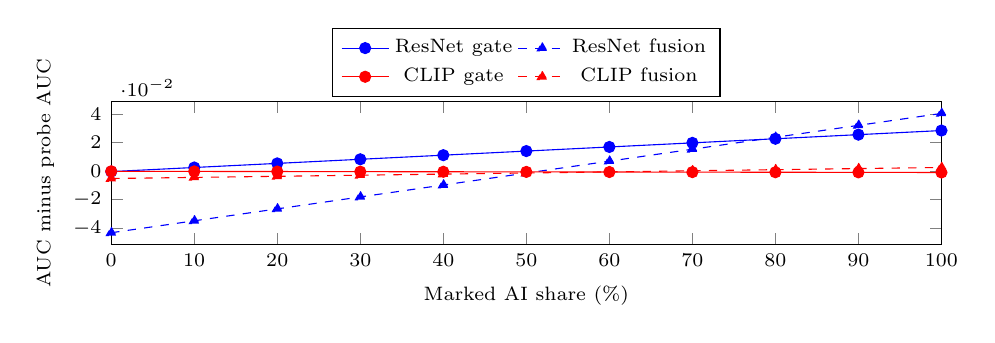
\begin{tikzpicture}
\begin{axis}[width=\columnwidth,height=3.4cm,xmin=0,xmax=100,
xlabel={Marked AI share (\%)},ylabel={AUC minus probe AUC},
tick label style={font=\scriptsize},label style={font=\scriptsize},
legend columns=2,legend style={font=\scriptsize,at={(0.5,1.03)},anchor=south}]
\addplot[blue,solid,mark=*] coordinates {(0,-0.0003002) (10,0.0025891) (20,0.0054784) (30,0.0083677) (40,0.0112570) (50,0.0141463) (60,0.0170356) (70,0.0199249) (80,0.0228142) (90,0.0257035) (100,0.0285928)};\addlegendentry{ResNet gate}
\addplot[blue,dashed,mark=triangle*] coordinates {(0,-0.0433280) (10,-0.0349308) (20,-0.0265336) (30,-0.0181363) (40,-0.0097391) (50,-0.0013419) (60,0.0070554) (70,0.0154526) (80,0.0238498) (90,0.0322471) (100,0.0406443)};\addlegendentry{ResNet fusion}
\addplot[red,solid,mark=*] coordinates {(0,-0.0000883) (10,-0.0001713) (20,-0.0002542) (30,-0.0003372) (40,-0.0004202) (50,-0.0005032) (60,-0.0005862) (70,-0.0006692) (80,-0.0007521) (90,-0.0008351) (100,-0.0009181)};\addlegendentry{CLIP gate}
\addplot[red,dashed,mark=triangle*] coordinates {(0,-0.0051657) (10,-0.0043880) (20,-0.0036104) (30,-0.0028328) (40,-0.0020552) (50,-0.0012775) (60,-0.0004999) (70,0.0002777) (80,0.0010553) (90,0.0018330) (100,0.0026106)};\addlegendentry{CLIP fusion}
\end{axis}\end{tikzpicture}
\caption{Unconditional and gated clean-image fusion gain. Repeats are weighted
counterfactual outcomes of the same 1,396 synthetic sources.}
\label{fig:prevalence}
\end{figure}

\subsection{Independent decision calibration}
Table~\ref{tab:calibration} shows the recall cost of source-max calibration
on the sixteen-condition test family.
Some realized source FPRs still exceed 0.05 (maximum 0.066);
CLIP S16 TPR split SD is 0.132. Source-max core13 calibration does not cover
the added weak views: CLIP source FPR rises to 0.111 on all16 versus 0.019
on core13. These measured costs and variability qualify the marginal claim.

\begin{table}[t]
\caption{Fixed probes with independent calibration on the original sixteen-condition
test family, mean$\pm$SD over five splits. I: thirteen-condition image target; S13/S16:
source-max cuts using thirteen/sixteen calibration conditions. Source FPR:
any positive copy per photographic source.}
\label{tab:calibration}\centering\footnotesize\setlength{\tabcolsep}{3pt}
\begin{tabular}{llccc}\toprule
Probe & Policy & Image TPR & Image FPR & Source FPR\\\midrule
ResNet & I & $0.733\pm0.026$ & $0.056\pm0.012$ & $0.215\pm0.025$\\
ResNet & S13 & $0.453\pm0.085$ & $0.010\pm0.007$ & $0.047\pm0.026$\\
ResNet & S16 & $0.402\pm0.046$ & $0.007\pm0.004$ & $0.035\pm0.015$\\
CLIP & I & $0.964\pm0.007$ & $0.097\pm0.015$ & $0.530\pm0.040$\\
CLIP & S13 & $0.821\pm0.052$ & $0.014\pm0.006$ & $0.111\pm0.044$\\
CLIP & S16 & $0.666\pm0.132$ & $0.005\pm0.003$ & $0.035\pm0.025$\\
\bottomrule\end{tabular}\end{table}

\subsection{Experiment 2: encoding and fresh sample}
Common PNG/JPEG95/75/50 gives ResNet AUC 0.958/0.955/0.952/0.952 and
CLIP 0.998/0.996/0.998/0.995 on 180 test pairs. Published
UniversalFakeDetect reaches native AUC 0.659 [0.583,0.733], versus 0.442
after common resizing/JPEG; the failure cause is unconfirmed.
On the locked 400-source replication, original unmarked identity probe AUC
is 0.965/0.994 (ResNet/CLIP). Across four edits, marked ResNet gate gain is
0.0144 [0.0090,0.0206], while unmarked gain is -0.0006 [-0.0012,-0.0001].
On the new caption-paired identity test, joint ResNet/CLIP AUC is
0.729/0.820; paired-bootstrap intervals are [0.686, 0.773]/[0.785, 0.855].
Joint CLIP JPEG50/low-res32 AUC is 0.795/0.696; its fixed image FPR is
0.020/0.325. All heads and cuts remain fixed.
The SD-out arm (Table~\ref{tab:paired}) changes the synthetic training mix as well as supervised
generator exposure; it is a restricted transfer control.
On these unmarked identity images, ResNet fusion/gate AUC is 0.664/0.730 (Fig.~\ref{fig:roc}).
Omitting three coarse-hash-flagged pairs post hoc gives joint ResNet/CLIP AUC 0.733/0.823; all 200 pairs remain primary.
Each joint probe has S16 identity FPR 0/200; its two-sided 95\% binomial upper bound is 0.0183 under independent common-risk source sampling.

\begin{figure}[t]
\centering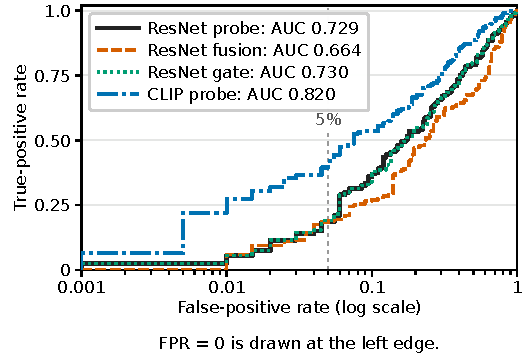
\includegraphics[width=\columnwidth]{assets/resnet_roc.pdf}
\caption{Frozen joint heads on the new unmarked caption-paired identity test,
200 real/AI pairs. Vertical line: 5\% FPR; zero-FPR points appear at the left
display edge. Fusion and gating use the classical expected payload.}
\label{fig:roc}\end{figure}
\begin{table}[t]
\caption{New unmarked caption pairs, identity primary endpoint; 200 pairs.
Joint: original full probe; SD-out: SD/Midjourney-excluded probe with
DALL$\cdot$E~3-only synthetic fitting. I/S16 use fixed image/source-max cuts.}
\label{tab:paired}\centering\footnotesize\setlength{\tabcolsep}{3pt}
\begin{tabular}{llrrrrr}\toprule
Probe & Fit & AUC & I TPR & I FPR & S16 TPR & S16 FPR\\\midrule
ResNet & Joint & 0.729 & 0.170 & 0.045 & 0.020 & 0.000\\
ResNet & SD-out & 0.654 & 0.110 & 0.055 & 0.000 & 0.000\\
CLIP & Joint & 0.820 & 0.310 & 0.020 & 0.025 & 0.000\\
CLIP & SD-out & 0.838 & 0.305 & 0.035 & 0.085 & 0.005\\
\bottomrule\end{tabular}\end{table}

\subsection{Experiment 3: learned mark}
Default positives use the first payload (Table~\ref{tab:modern});
any-three positives average all three payload covers.
Across four views, default-query photographic false-match rates are
0.047/0.054 (DWT--DCT/TrustMark), with source-bootstrap intervals
[0.034, 0.061]/[0.043, 0.065].
The separately calibrated any-three rule gives marked-AI acceptance
0.475/0.906 and photographic false matches 0.054/0.035.
Default-query unmarked-AI false matches are
0.050/0.042; photographic calibration does not guarantee AI false-match rates.
For any zero-event photographic collection, 0/200 has a two-sided 95\% binomial upper bound 0.0183 under independent common-risk sources; zero bootstrap intervals are degenerate.
TrustMark low-res32 margin acceptance is 136/204, but full expected-message/schema/ECC recovery is only 5/204; partial information-bit evidence does not imply message recovery.

\begin{table}[t]
\caption{Matched 40\,dB embeddings and 16 information bits, default query.
Separate thresholds target calibration FPR$\le5\%$; test FPR need not equal.
TPR: margin acceptance on 204 marked AI, not full-message recovery;
FP: 400 unmarked photographs. D: DWT--DCT; T: TrustMark.}
\label{tab:modern}\centering\footnotesize\setlength{\tabcolsep}{3pt}
\begin{tabular}{lrrrr}\toprule
Condition & D TPR & T TPR & D FP & T FP\\\midrule
Identity & 0.980 & 1.000 & 0.060 & 0.060\\
JPEG50 & 0.951 & 0.995 & 0.068 & 0.060\\
Crop & 0.059 & 1.000 & 0.060 & 0.040\\
Low-res32 & 0.000 & 0.667 & 0.000 & 0.055\\
\bottomrule\end{tabular}\end{table}
The original embedding/verification criteria give diffusion 0.50 recovery
6/204 for DWT--DCT [0.011,0.063] and 0/204 for TrustMark [0.000,0.018].
Realistic Vision DDIM uses twenty configured steps (ten effective), empty
prompt, guidance one and fixed seed; PSNR against marked input is 16.1/16.1\,dB.
These highly distorted, marked-AI-only reconstructions supplement the fair
comparison and do not establish robustness under content-preserving removal.

\section{Discussion and Limitations}
Unequal augmentation distortion/information and restricted fitting prevent
attributing full-suite gains to matching alone. Gating improves marked ResNet
ranking but can slightly harm unmarked inputs. Caption pairing and generation
change jointly, preventing attribution of poor transfer to content alone.
Source-max cuts sacrifice recall; their marginal assumptions do not guarantee
deployment error rates.

Core controls and calibration reanalyses are retrospective; the caption test
uses prospectively fixed policies. Splits share sources, and intervals
condition on fitted models. Prefix sampling, unverified generator labels,
original compression, resolution, scene content, and pretraining overlap
remain confounds. Caption pairing aligns descriptions, not identical scenes;
one LCM-accelerated SD1.5-family pipeline does not establish unseen-family
generalization. Shared final JPEG encoding cannot undo earlier processing.
Hash screening can miss semantic duplicates or exclude distinct scenes.
Postgeneration checks found no exact matches, but three generated images have
coarse hash similarities to prior records; all remain in the locked primary test.

Both marks lack issuer authentication; the classical public payload is
unkeyed. Independent uniform bits would pass 13/16 with probability
$697/65536\approx0.0106$, but measured bits may be dependent.
Common information bits/distortion/nominal target do not equalize embedding
redundancy, official decoding semantics, or test FPR. Residual scaling and
stochastic rounding modify official embeddings. One diffusion checkpoint,
adaptive published removal, Stable Signature, Tree-Rings, recapture, and
external benchmark transfer remain scope limits.

\section{Reproducibility}
The cleaned anonymous code and aggregate evidence are prepared locally; public hosting is pending.
No benchmark images, private metadata, embeddings or weights are released;
code, public indices, protocols and aggregate fingerprints support reproduction.

\section{Conclusion}
Processing controls yield modest matching gains and conditional fusion
benefits, with limited caption-paired transfer. Calibration and matched
watermark operating points quantify false-alarm/recall and recovery limits
within the tested scope.
\balance
\section*{Acknowledgment}
OpenAI Codex assisted drafting/revising Sections I--VIII, analysis/plotting
code and primary-reference lookup. OpenAI's image-generation
tool supplied Fig.~\ref{fig:pipeline}'s illustration; study algorithms
produced its edits. Numerical results use archived outputs.
\begin{thebibliography}{99}
\bibitem{univfd}
U.~Ojha, Y.~Li, and Y.~J. Lee, ``Towards universal fake image detectors that generalize across generative models,'' in \emph{Proc. IEEE/CVF Conf. Comput. Vis. Pattern Recognit. (CVPR)}, 2023, pp.~24480--24489.


\bibitem{genimage}
M.~Zhu \emph{et al.}, ``{GenImage}: A million-scale benchmark for detecting {AI}-generated image,'' in \emph{Adv. Neural Inf. Process. Syst.}, vol.~36, 2023.


\bibitem{zhao}
X.~Zhao \emph{et al.}, ``Invisible image watermarks are provably removable using generative {AI},'' in \emph{Adv. Neural Inf. Process. Syst.}, vol.~37, 2024.


\bibitem{unmarker}
A.~Kassis and U.~Hengartner, ``{UnMarker}: A universal attack on defensive image watermarking,'' in \emph{Proc. IEEE Symp. Security Privacy}, 2025, doi:~10.1109/SP61157.2025.00005.


\bibitem{cnndetect}
S.-Y.~Wang, O.~Wang, R.~Zhang, A.~Owens, and A.~A. Efros, ``{CNN}-generated images are surprisingly easy to spot\ldots\ for now,'' in \emph{Proc. IEEE/CVF Conf. Comput. Vis. Pattern Recognit. (CVPR)}, 2020.


\bibitem{dire}
Z.~Wang \emph{et al.}, ``{DIRE} for diffusion-generated image detection,'' in \emph{Proc. IEEE/CVF Int. Conf. Comput. Vis. (ICCV)}, 2023, pp.~22445--22455.


\bibitem{cifake}
J.~J. Bird and A.~Lotfi, ``{CIFAKE}: Image classification and explainable identification of {AI}-generated synthetic images,'' \emph{IEEE Access}, vol.~12, pp.~15642--15650, 2024, doi:~10.1109/ACCESS.2024.3356122.


\bibitem{ldm}
R.~Rombach, A.~Blattmann, D.~Lorenz, P.~Esser, and B.~Ommer, ``High-resolution image synthesis with latent diffusion models,'' in \emph{Proc. IEEE/CVF Conf. Comput. Vis. Pattern Recognit. (CVPR)}, 2022, pp.~10684--10695.


\bibitem{sdedit}
C.~Meng \emph{et al.}, ``{SDEdit}: Guided image synthesis and editing with stochastic differential equations,'' in \emph{Proc. Int. Conf. Learn. Represent. (ICLR)}, 2022.


\bibitem{trustmark}
T.~Bui, S.~Agarwal, and J.~Collomosse, ``{TrustMark}: Robust watermarking and watermark removal for arbitrary resolution images,'' in \emph{Proc. IEEE/CVF Int. Conf. Comput. Vis. (ICCV)}, 2025, pp.~18629--18639.


\bibitem{signature}
P.~Fernandez, G.~Couairon, H.~J\'egou, M.~Douze, and T.~Furon, ``The stable signature: Rooting watermarks in latent diffusion models,'' in \emph{Proc. IEEE/CVF Int. Conf. Comput. Vis. (ICCV)}, 2023, pp.~22466--22477.


\bibitem{treering}
Y.~Wen, J.~Kirchenbauer, J.~Geiping, and T.~Goldstein, ``Tree-rings watermarks: Invisible fingerprints for diffusion images,'' in \emph{Adv. Neural Inf. Process. Syst.}, vol.~36, 2023.


\bibitem{alhaj}
A.~Al-Haj, ``Combined {DWT-DCT} digital image watermarking,'' \emph{J. Comput. Sci.}, vol.~3, no.~9, pp.~740--746, 2007, doi:~10.3844/jcssp.2007.740.746.


\bibitem{advmark}
X.~Wu, X.~Liao, B.~Ou, Y.~Liu, and Z.~Qin, ``Are watermarks bugs for deepfake detectors? Rethinking proactive forensics,'' in \emph{Proc. 33rd Int. Joint Conf. Artif. Intell. (IJCAI)}, 2024, pp.~6089--6097, doi:~10.24963/ijcai.2024/673.


\bibitem{nist}
B.~Chandra, J.~Dunietz, K.~Roberts, Y.~Lee, P.~Fontana, and G.~Awad, ``Reducing risks posed by synthetic content: An overview of technical approaches to digital content transparency,'' Nat. Inst. Standards Technol., NIST AI 100-4, 2024, doi:~10.6028/NIST.AI.100-4.


\bibitem{coco}
T.-Y.~Lin \emph{et al.}, ``Microsoft {COCO}: Common objects in context,'' in \emph{Proc. Eur. Conf. Comput. Vis. (ECCV)}, 2014, pp.~740--755.


\bibitem{diffusiondb}
Z.~J. Wang, E.~Montoya, D.~Munechika, H.~Yang, B.~Hoover, and D.~H. Chau, ``{DiffusionDB}: A large-scale prompt gallery dataset for text-to-image generative models,'' in \emph{Proc. 61st Annu. Meeting Assoc. Comput. Linguistics}, 2023, pp.~893--911, doi:~10.18653/v1/2023.acl-long.51.


\bibitem{dalle}
ehristoforu, ``{DALL}$\cdot${E}~3 images,'' Hugging Face dataset, accessed Oct.~7, 2026. [Online]. Available: \url{https://huggingface.co/datasets/ehristoforu/dalle-3-images}


\bibitem{midjourney}
D.~Sharma, ``{AI} generated images: {Midjourney},'' Hugging Face dataset, accessed Oct.~7, 2026. [Online]. Available: \url{https://huggingface.co/datasets/ideepankarsharma2003/AIGeneratedImages_Midjourney}


\bibitem{openimages}
A.~Kuznetsova \emph{et al.}, ``The {Open Images} dataset {V4}: Unified image classification, object detection, and visual relationship detection at scale,'' \emph{Int. J. Comput. Vis.}, 2020.


\bibitem{lcm}
S.~Luo \emph{et al.}, ``{LCM-LoRA}: A universal stable-diffusion acceleration module,'' arXiv:2311.05556, 2023.

\bibitem{resnet}
K.~He, X.~Zhang, S.~Ren, and J.~Sun, ``Deep residual learning for image recognition,'' in \emph{Proc. IEEE Conf. Comput. Vis. Pattern Recognit. (CVPR)}, 2016, pp.~770--778.


\bibitem{clip}
A.~Radford \emph{et al.}, ``Learning transferable visual models from natural language supervision,'' in \emph{Proc. 38th Int. Conf. Mach. Learn.}, vol.~139, 2021, pp.~8748--8763.


\bibitem{conformal}
A.~N. Angelopoulos and S.~Bates, ``A gentle introduction to conformal prediction and distribution-free uncertainty quantification,'' arXiv:2107.07511v6, 2022.

\end{thebibliography}\end{document}
